\documentclass[12pt]{article}
\usepackage[margin=0.75in]{geometry}
\usepackage{graphicx}
\usepackage{amsmath,amsthm,amssymb,amsfonts, bm}
\usepackage{enumitem, nth}
\usepackage{mathtools}

\usepackage{listings}
\usepackage{color}
 
\definecolor{codegreen}{rgb}{0,0.6,0}
\definecolor{codegray}{rgb}{0.5,0.5,0.5}
\definecolor{codepurple}{rgb}{0.58,0,0.82}
\definecolor{backcolour}{rgb}{0.95,0.95,0.92}
 
\lstdefinestyle{mystyle}{
    backgroundcolor=\color{backcolour},   
    commentstyle=\color{codegreen},
    keywordstyle=\color{magenta},
    numberstyle=\tiny\color{codegray},
    stringstyle=\color{codepurple},
    basicstyle=\footnotesize,
    breakatwhitespace=false,         
    breaklines=true,                 
    captionpos=b,                    
    keepspaces=true,                 
    numbers=left,                    
    numbersep=5pt,                  
    showspaces=false,                
    showstringspaces=false,
    showtabs=false,                  
    tabsize=4
}
 
\lstset{style=mystyle}


\begin{document}
\title{CS224n HW1}
\author{Xinyu Tan}
\maketitle

%-----------------------------
% problem 1: softmax
%-----------------------------
\section {Softmax}
\subsection*{(a)}
Take a look at any element $i$, 
$$
\text{softmax}(\bm x + c)_i = \frac{e^{\bm x_i + c}}{\sum_{j} e^ {\bm x_j + c}} = \frac{e^c \cdot e^{\bm x_i}}{e^c \cdot \sum_j e^{\bm x_j}} = \text{softmax}(\bm x )_i 
$$
Therefore, we have $\text{softmax}(\bm x + c) = \text{softmax}(\bm x)$

\subsection*{(b)}
Note the first case illustrate the broadcasting principle (dimension match) in numpy:
\begin{lstlisting}[language=Python]
if len(x.shape) > 1:
	#matrix
	x = x - np.max(x, axis=1, keepdims=True)
	x = np.exp(x) / np.sum(np.exp(x), axis=1, keepdims=True)
else:
	# vector
	x = x - x.max() # normalize
	x = np.exp(x)/np.sum(np.exp(x))
\end{lstlisting}


%----------------------------------------------
% problem 2: Neural network basics
%----------------------------------------------
\section{Neural Network Basics}
\subsection*{(a)}
$$
\frac{d \sigma (x)}{dx} = \frac{e^{-x}}{(1-e^{-x})^2} = \sigma(x) (1 - \sigma(x))
$$

\subsection*{(b)}
First, we have
	$$\hat y_i = \frac{e^{\theta_i}}{\sum_j e^{\theta_j}}$$
For one-hot encoding, only $k$-th element in $\bm y$ is \emph{one}, so we have
\begin{align*}
CE(\bm y, \bm {\hat y}) &= - \log \hat y_k = - \log \frac{e^{\theta_k}}{\sum_j e^{\theta_j}} \\
				&= - \theta_k + \log \sum_j e^{\theta_j}
\end{align*}

Therefore, 
\begin{align*}
&\frac{\partial CE(\bm y, \bm {\hat y})} {\partial \theta_k} = -1 + \frac{e^{\theta_k}}{\sum_j e^{\theta_j}}  \\
&\frac{\partial CE(\bm y, \bm {\hat y})} {\partial \theta_i} =  \frac{e^{\theta_i}}{\sum_j e^{\theta_j}}, \forall i \neq k
\end{align*}

Put them altogether,
$$
\frac{\partial CE(\bm y, \bm {\hat y})} {\partial \bm \theta} = -\bm y + \text{softmax}(\bm {\theta}) = \bm {\hat y} - \bm y
$$

\subsection*{(c)}
We have 
\begin{align*}
\bm {\hat y} &= \text{softmax}(\bm h \bm W_2 + \bm b_2) \\
	           &= \text{softmax} \left ( \text{sigmoid} (\bm x \bm W_1 + \bm b_1)  + \bm b_2\right)
\end{align*}
Denote $\bm a_2 = \bm h \bm W_2 + \bm b_2$ and $\bm a_1 = \bm x \bm W_1 + \bm b_1$, then 
\begin{align*}
\frac{\partial CE(\bm y, \bm {\hat y})} {\partial \bm x} &=  \frac{\partial CE(\bm y, \bm {\hat y})}{\partial \bm a_2} \frac{\partial \bm a_2}{\partial \bm x} \\
&=  (\bm {\hat y} - \bm y) \frac{\partial \bm a_2}{\partial \bm h} \frac{\partial \bm h} {\partial \bm x} \\
&= (\bm {\hat y} - \bm y) \bm W_2^T \sigma'(\bm a_1) \bm W_1^T
\end{align*}

\subsection*{(d)}

There are in total $D_x H + H +H D_y+Dy$ parameters.


%----------------------------------------------
% problem 3: word2vec
%----------------------------------------------
\section{word2vec}

\subsection*{(a)}	
For a word $\bm o$, the loss function is
\begin{align*}
L &= -y_o \log {\hat y_o} = -\log {\frac{\exp(\bm u_o^T \bm v_c)} {\sum_{w=1}^W \exp(\bm u_w^T \bm v_c)}} \\
   &= -\bm u_o^T \bm v_c + \log{\sum_{w=1}^W \exp(\bm u_w^T \bm v_c})
\end{align*}

Therefore, derivative with respect to $\bm v_c$ is:
\begin{align*}
\frac{\partial L}{\partial \bm v_c} &= -\bm u_o + \frac{1}{\sum_{l=1}^{W} \exp( \bm u_l^T \bm v_c)} \sum_{w=1}^{W} \exp(\bm u_w^T \bm v_c) \bm u_w \\
&= -\bm u_o + \sum_{w=1}^W p(w|c) \bm u_w
\end{align*}
where $$p(w|c) = \frac{\exp(\bm u_w^T \bm v_c)}{\sum_{l=1}^{W} \exp( \bm u_l^T \bm v_c)}$$.


\subsection*{(b)}
Similarly,

$$
\frac{\partial L}{\partial \bm u_w} = \begin{cases}
						- (1 - \hat y_o)\bm v_c ( & w =o \\
						\hat y_w \bm v_c  & w \neq o
						     \end{cases}
$$

\subsection*{(c)}
Given $$J_{\text{neg-sample}}(\bm o, \bm v_c, \bm U) = -\log \sigma (\bm u_o^T \bm v_c) - \sum_{k=1}^K \log \sigma (-\bm u_o^T \bm v_c) $$
we have 
\begin{align*}
\frac{\partial J}{\partial \bm v_c} = - \sigma (-\bm u_o^T \bm v_c) \bm u_o + \sum_{k=1}^K \sigma(\bm u_k^T \bm v_c) \bm u_k
\end{align*}
and
$$
\frac{\partial J}{\partial \bm u_w} = \begin{cases}
					-\sigma(-\bm u_w^T \bm v_c)\bm v_c & w = o \\
					\sigma(\bm u_w^T \bm v_c)\bm v_c & w \neq o
					\end{cases}
$$

\subsection*{(d)}
Let's denote $\bm U$ the matrix that aggregates all the output word vectors. 

\begin{enumerate}
\item Skip-gram: 
	$$\frac{\partial J_\text{skip-gram}}{\partial \bm U} = \sum_{j\neq0} \frac{\partial F(\bm u_{c+j}, \bm v_c)}{\partial \bm U}$$ 
	$$\frac{\partial J_\text{skip-gram}}{\partial \bm v_c} =  \sum_{j\neq0} \frac{\partial F(\bm u_{c+j}, \bm v_c)}{\partial \bm v_c}$$
\item CBOW: 
	$$\frac{\partial J_\text{CBOW}}{\partial \bm U} = \frac{\partial F(\bm u_{c}, \bm{\hat v})}{\partial \bm U}$$
	$$\frac{\partial J_\text{CBOW}}{\partial \bm v_j} = \frac{\partial F(\bm u_{c}, \bm{\hat v})}{\partial \bm{\hat v}}$$ 
\end{enumerate}

\subsection*{(g)}

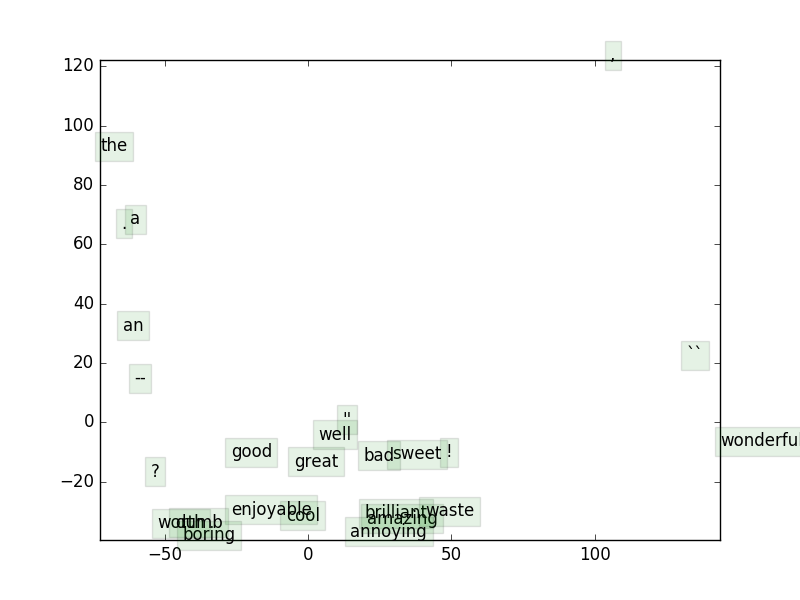
\includegraphics[scale=0.8]{../assignment1/q3_word_vectors.png}

Summary: ``the'', ``a'', and ``an'' are close to each other; most adjectives are clustered at the bottom of the graph; ``wonderful'' somehow is far from its similar words. 

%----------------------------------------------
% problem 4: Sentiment Analysis
%----------------------------------------------
\section{Sentiment Analysis}

\subsection*{(b)}
The main reason to introduce regularization is to avoid overfitting. 

\subsection*{(c)}
Code for choosing the best model:
\begin{lstlisting}[language=Python]
def chooseBestModel(results):
    """Choose the best model based on parameter tuning on the dev set

    Arguments:
    results -- A list of python dictionaries of the following format:
        {
            "reg": regularization,
            "clf": classifier,
            "train": trainAccuracy,
            "dev": devAccuracy,
            "test": testAccuracy
        }

    Returns:
    Your chosen result dictionary.
    """
    bestResult = None

    ### YOUR CODE HERE
    test_acc = []
    for res in results:
        test_acc.append(res["dev"])
    ### END YOUR CODE
    best_index = test_acc.index(max(test_acc))
    bestResult = results[best_index]
    return bestResult
\end{lstlisting}



\end{document}